\documentclass[letterpaper, 10 pt, conference]{ieeeconf}

\usepackage{algorithm}
\usepackage[noend]{algpseudocode}
\usepackage{bm}

\usepackage{amsfonts}
\usepackage[pdftex]{graphicx}
\usepackage{comment}

\usepackage{caption}
\usepackage{subcaption}

%\usepackage{amsthm}
\newtheorem{thm}{Theorem}
\newtheorem{lem}{Lemma}
%\newtheorem{asmp}{Assumption}
\newtheorem{defn}{Definition}
%\newtheorem{clm}{Claim}

\IEEEoverridecommandlockouts                              % This command is only needed if 
                                                          % you want to use the \thanks command

\overrideIEEEmargins                                      % Needed to meet printer requirements.

\title{\LARGE \bf
Homotopy-aware RRT$^{*}$ : Toward optimal path planning with the consideration of the topology
}

\author{
Daqing Yi, Michael A. Goodrich and Kevin D. Seppi
\thanks{Daqing Yi, Michael A. Goodrich and Kevin D. Seppi are with Department of Computer Science, Brigham Young University, Provo, UT, 84604, USA.
{\tt\small daqing.yi@byu.edu, mike@cs.byu.edu, kseppi@cs.byu.edu} }
}

\begin{document}


\maketitle
\thispagestyle{empty}
\pagestyle{empty}


%%%%%%%%%%%%%%%%%%%%%%%%%%%%%%%%%%%%%%%%%%%%%%%%%%%%%%%%%%%%%%%%%%%%%%%%%%%%%%%%
\begin{abstract}
The topology factor of the paths is often ignored in the task planning.
Because it is difficult to be modeled in the optimal motion planning problems, especially when it is not a hard constraint.
In plenty of the tasks, the goal is not only to optimize some objective, i.e. ``go quickly from A to B avoiding C'', but also contains some topological constraints.
In this paper, we propose HA-RRT$^{*}$, a homotopy-aware RRT$^{*}$, that explores the planning space for optimal solutions with the consideration of the topology of the paths.
Because the algorithm is aware of the homotopy classes of each branch, it can support sliding autonomy for different levels of human's intent on the path topology.
Thus, a clear intent on the path topology provides the homotopic constraint, which reduces the working space of the optimal search;
a vague intent on the path topology can be identified by comparing the optimal solutions in different homotopy classes.
We provides the applications to show how it works in different cases and the corresponding theoretic analyses.
\end{abstract}

\begin{comment}
six pages
\end{comment}

%%%%%%%%%%%%%%%%%%%%%%%%%%%%%%%%%%%%%%%%%%%%%%%%%%%%%%%%%%%%%%%%%%%%%%%%%%%%%%%%
\section{Introduction}
\label{sec:intro}

Optimality has been the most important heuristic in planning motions for the robots.
An optimization problem is usually modeled by using the metric that measures the task performance.
As the task supervisor, it is very essential that the human's intent can be correctly and precisely modeled into the optimization problem.
Thus, the planned solution for the robot can be the one matches the human's intent.
In planning the robot's motion in a task, the most common way of modeling the intent is by defining single objective~\cite{6974170} or multiple objectives~\cite{yi2014supporting}.
The generated path is a solution that optimizes the given objectives, for example, minimizing the Euclidean distance.
Not all types of the human's intents can be easily modeled using measurable objectives.
The ``shape'' of the planned path, which indicates the topology in the environments with complex obstacles, is one of them.
Such intent can be a hope of avoiding visiting some regions, a will of moving around some objects or a preference of how the motion is like.
Some of the intents are defined as constraints, for example via-point constraint, reference path constraint~\cite{6974170} or temporal logic constraint~\cite{5650896}, in the optimization problems.
This method won't work when there is only preference on the ``shape'' of the paths instead of hard constraint.
At the same time, the preference on the ``shape'' of the paths might also be fuzzy for the human to describe.

\emph{Homotopy} is commonly used to indicate the inherent topological similarity of the paths.
Given two paths, if one can be deformed into the other without encroaching any obstacle, they are said to be \emph{homotopic}~\cite{Hernandez201544}.
Thus, we can have a \emph{homotopy class}, in which any two paths are homotopic.
Given the start position and the end position, the obstacles in the map can determine several homotopy classes.
The homotopy of the paths can then be used for modeling the human's intent on the path ``shape''. 


Now in a path planning problem, a human task supervisor is defining a task for a robot.
The task is needed to be modeled so that the robot can understand and plan for execution.
Assume the objective is only reaching to a target quickly, there can be several levels of how clear his intent is.
\begin{enumerate}
\item \emph{I only want the planned path sequentially visiting several regions.}
It means that the planned path is constrained in one homotopy class.
The homotopy class becomes the constraint of the optimization problem~\cite{Hershberger199463}.
%This homotopy class could be defined from a human initialized reference path.
\item \emph{I know some regions that have to be visited and some regions could not be reached.}
There can exist several homotopy classes that can satisfy the requirement defined by the required regions and forbidden regions.
In this case, the homotopic constraint becomes several homotopy classes instead of only one.
\item \emph{I feel some path ``shape'' is better when comparing with another ``shape''.}
It indicates that the human has preference on different homotopy classes.
If the preference on the homotopy classes can be modeled as one objective, the non-dominant solutions can be found.
Thus the human could select one from the Pareto optimal paths.
\item \emph{I should have preference but it is hard for me to tell.}
In this case, the human's preference could be identified through interactive process.
Another straightforward way is that the planning algorithm provides the best solution of each homotopy class to the supervisor.
The supervisor can then select one that satisfy his/her intent.
\end{enumerate}

In this paper, we propose a homotopy-aware RRT$^{*}$ that awares the homotopy class each branch belongs to while exploring the planning space by optimal heuristic.
It could assist the planner finding the intended optimal path in considering the homotopy.
We review the relevant work in section \ref{sec:related_work}.
We introduce the algorithm in section \ref{sec:algorithm} and analyze the algorithm in section \ref{sec:analysis}.
The proposed algorithm is applied into different level of sliding autonomy in section \ref{sec:application}.

\section{Related work}
\label{sec:related_work}

Homotopy reveals the similarity between two paths.
It can be used to determine the similarity between a reference path and a normal path, or classify the paths into different classes.
Homotopy-based path planning depends on the determination of the homotopy equivalence of two paths, which is usually computationally expensive.

Voronoi diagram is naturally introduced to assist determining the homotopy classes, but it shows limitation on finding some paths in some cases~\cite{banerjee2013framework}.
Particularly, generating Voronoi diagram for obstacles of complicated shapes is hard.
By algebraic topology, the path of same homotopy class can be determined by using orientable band~\cite{Hershberger199463}.
Similarly, the problem and complexity come when the shapes of the obstacles are not smooth and convex.
Semi-algebraic cuts are used to converting the path into ``word'' so that the homotopic equivalence can be compared~\cite{Grigoriev:1998:PAS:281508.281528}.
The Cauchy Integral theorem has been introduced to determine homotopy class by marking the positions in the obstacles as undefined~\cite{AAAI101920}.
Because the map is discretized, the computation cost expands greatly if the obstacles are reasonably approximated by the cells.

Sampling-based path planning has been an effective and popular tool.
The idea of homotopy has also been imported here.
By homotopic redundancy, the paths from PRM could be compared by the homotopy classes~\cite{1041613}.
By dividing the space using the rays crossing each obstacle, reference frames could be used to represent the paths into canonical sequences~\cite{Hernandez201544}.
In this way, the extending process of the graph structure keeps tracking the homotopy class of the new branch so that the exploration process can be constrained by some homotopy classes.

In order to accelerate the exploration process, bidirectional RRT has been introduced to accelerate the exploration process.
In the optimal sampling process, the optimality is still preserved~
\cite{Jordan.Perez.ea:CSAIL13}~\cite{starek2014bidirectional}.
With two trees exploring from two directions, we can have the optimal cost-to-go and the optimal cost-to-arrive at different position.
This guarantee the optimality search with the homotopical constraint.
We introduce the homotopy-aware bidirectional RRT$^{*}$ to support different level of intent on topology from the planner.

\section{Homotopy-aware RRT$^{*}$}
\label{sec:algorithm}

Without loss of generality, we look at a minimization problem.
We can have the definition of homotopy-based optimal path planning problem.
It can be extended into many homotopy-relevant optimal path planning.
\begin{defn}{ \textbf{Homotopy-based optimal Path Planning} }
Consider a bounded, connected open set $ X \subset \mathbb{R}^{d} $, an obstacle space $ X_{obs} $, an initial state $ x_{init} $, and a goal state $ x_{goal} $. 
Denote the obstacle-free space by $ X_{\it free} = X \setminus X_{obs} $.
Define a {\em path} in $X$ as a continuous curve parameterized by $s$, denoted by $\sigma : [0,s] \rightarrow X$. 
Define the cost of the path as the vector-valued function $ {\sc Cost} (\sigma) $.  
The goal is to find paths $ \sigma^{*} \in \Sigma^{*}$ such that
\textit{ (a) }, $\forall \tau\in[0,s], \sigma^*(\tau) \in X_{\it free}$;
\textit{ (b) }, $ \sigma^{*} (0) = x_{init} $ and $ \sigma^{*} (s) = x_{goal}  $;
\textit{ (c) }, $ \sigma^{*} = \min_{\sigma \in X_{\it free} } {\sc Cost} (\sigma) $ with given homotopy constraints.
\end{defn} 

We adopt the Jenkin's method~\cite{Hernandez201544} to generate reference frames given a map with obstacles.
The map is decomposed into several regions by the lines connecting the center point and points in each obstacles.
The line segments, two ends of which connect with obstacles, are defined as \emph{reference frames}.
The topology of the path can be identified by how the sequence of crossing the reference frames is.
With the generated reference frames, we could import the bidirectional RRT$^{*}$ to accomplish the homotopy-aware exploration process.
The generation process of the reference frames is given in Algorithm \ref{alg:harrt:init_ref_frames}.

\begin{algorithm}[hbtp]
	\begin{algorithmic}[1]
		\State $ \bm{R} = \emptyset $
		\For{\textbf{each} $ B_{k} \in \bm{B} $ }
			\State $ b_{k} $ $ \leftarrow $ Sample from $ B_{k} $
			\State $ \bm{b} \leftarrow \bm{b} \cup b_{k} $
		\EndFor
		\While{ $ \exists b_{k}, b_{k'} , c \in $ \Call{Line}{ $ b_{k}, b_{k'} $ } }
			\State $ c \leftarrow  $ Sample from $ \bm{X}_{free} $
		\EndWhile
		\For{\textbf{each} $ b_{k} \in \bm{b} $ }
			\State $ \alpha_{k} \leftarrow $ \Call{Ray}{ $ b_{k}, c - b_{k} $ }
			\State $ \beta_{k} \leftarrow $ \Call{Ray}{ $ b_{k}, b_{k} - c $ }
			\State $ \bm{\alpha} \leftarrow \bm{\alpha} \cup \alpha_{k} $
			\State $ \bm{\beta} \leftarrow \bm{\beta} \cup \beta_{k} $			
		\EndFor
		\For{\textbf{each} $ \alpha_{k} \in \bm{\alpha} $}
			\State $ \{ \alpha_{k_{m}} \} \leftarrow $ \Call{Intersect}{$ \alpha_{k}, \bm{B} $}
			\State $ \bm{R} \leftarrow \bm{R} \cup \{ \alpha_{k_{m}} \} $
		\EndFor
		\For{\textbf{each} $ \beta_{k} \in \bm{\beta} $}
			\State $ \{ \beta_{k_{m}} \} \leftarrow $ \Call{Intersect}{$ \beta_{k}, \bm{B} $}
			\State $ \bm{R} \leftarrow \bm{R} \cup \{ \beta_{k_{m}} \} $
		\EndFor
		\Return $ \bm{R} $
	\end{algorithmic}
	\caption{ \textsc{InitRefFrames} ($ \bm{X}_{free} , \bm{B} $) }
	\label{alg:harrt:init_ref_frames}
\end{algorithm} 

\begin{figure}
	\centering
	\begin{subfigure}[t]{0.45\linewidth}
		\centering
		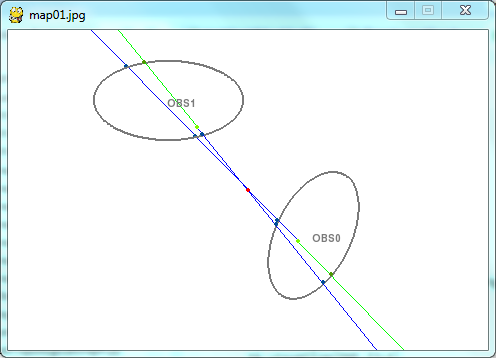
\includegraphics[width=\textwidth]{fig/obs_map.png}
		\caption{Decomposition of the map with obstacles.}
		\label{fig:obs_map:map}
	\end{subfigure}  
	%\\
	\begin{subfigure}[t]{0.5\linewidth}
		\centering
		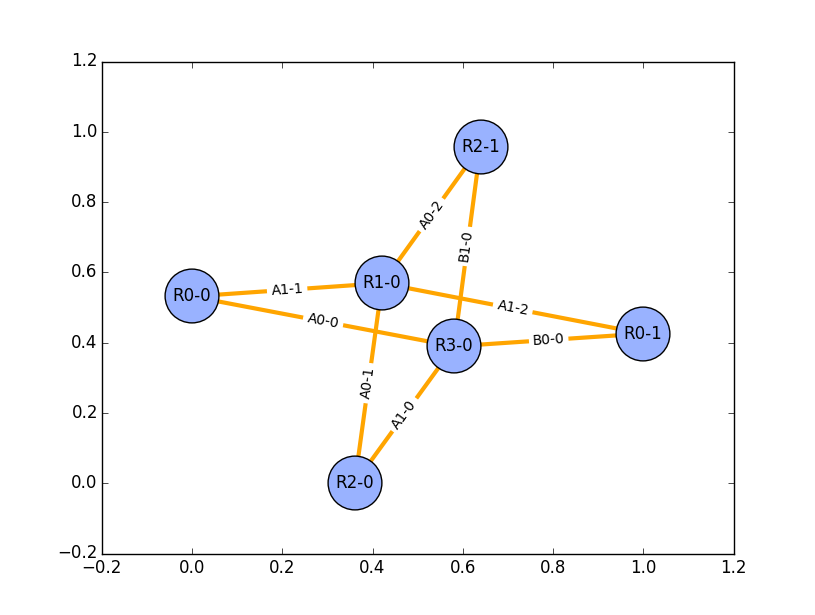
\includegraphics[width=\textwidth]{fig/obs_topology.png}
		\caption{The generated topological graph.}
		\label{fig:obs_map:topology}
	\end{subfigure}   
	\caption{Map with obstacles.}
	\label{fig:obs_map}
\end{figure}

\begin{itemize}
	\item \textsc{Line}($ p_{1}, p_{2} $):
	Return a line that defined by $ p_{1} $ and $ p_{2} $.
	\item \textsc{Ray}($ p, \vec{d} $):
	Return a ray that starts from $ p $ with direction $ \vec{d}  $.
	\item \textsc{Intersect}( $ r , \bm{B} $ ):
	Return line segments that a line $ r $ cut by the obstacles in $ B $.
\end{itemize}

After the reference frames $ \mathbf{R} $ are generated, we could have bidirectional RRT$^{*}$ explore the search space.
The process is given in Algorithm \ref{alg:harrt}.
Two trees $ G_{s} $ and $ G_{g} $ are constructed from $ x_{init} $ and $ x_{goal} $ respectively.
Two trees explore the map bidirectionally by calling {\sc Explore}(), defined in Algorithm \ref{alg:harrt:explore}, at each iteration.
At the end, paths are obtained by {\sc ExtractPaths}() from combining results of both two trees.

\begin{algorithm}
	\begin{algorithmic}[1]
		\State $ i \leftarrow 0 $
		\State $ V_{s} \leftarrow \{ x_{init} \} $; $ E_{s} \leftarrow \emptyset $; $ G_{s} \leftarrow (V_{s}, E_{s}) $
		\State $ V_{g} \leftarrow \{ x_{goal} \} $; $ E_{g} \leftarrow \emptyset $; $ G_{g} \leftarrow (V_{g}, E_{g}) $
		\While{ $ i < N $ }
			\State $ G_{s} \leftarrow $ \Call{Explore}{$ G_{s}, i $}
			\State $ G_{g} \leftarrow $ \Call{Explore}{$ G_{g}, i $}
			\State $ i \leftarrow i + 1 $
		\EndWhile
		\State \Call{ExtractPaths}{$ G_{s}, G_{g} $}
	\end{algorithmic}
	\caption{HA-RRT$^{*}$ ($ x_{init} , x_{goal}  $) }
	\label{alg:harrt}
\end{algorithm}

\begin{algorithm}
	\begin{algorithmic}[1]
		\State $ x_{rand} \leftarrow $ \Call{ Sample }{$ i $} ;
		\State $ x_{nearest} \leftarrow $ \Call{Nearest}{$ G, x_{rand} $}
		\State $ x_{new} \leftarrow $ \Call{Steer}{$ x_{nearest}, x_{rand},\eta $}
		\If{ \Call{ObstacleFree}{$ x_{nearest}, x_{new} $} }
			\State $ G \leftarrow $ \Call{ Extend }{$ G, x_{new}, x_{\it nearest} $}
		\EndIf
		\Return $ G $
	\end{algorithmic}
	\caption{ \textsc{Explore}($ G, i $) }
	\label{alg:harrt:explore}
\end{algorithm}

The {\sc Extend} procedure is inherited from the same method in \cite{Karaman-RSS-10}.
It is given in Algorithm \ref{alg:harrt:extend}.
The {\sc HomotopyCheck}() is added to guarantee that adding new edge or rewiring edges all satisfies the homotopy constraint.
The homotopy constraint is defined as a \emph{homotopic grammar}.
Because RRT$^{*}$ maintains a tree structure, each vertex has only one path to arrive from the root.
This path, which starts from the root to the vertex, indicates a string of characters sequentially.
Each character represents a crossed reference frame.
In the {\sc Extend} procedure, the {\sc HomotopyCheck}() uses a state machine to check whether the string satisfies the defined grammar.

\begin{algorithm}
	\begin{algorithmic}[1]
		\State $ V' \leftarrow V $; $ E' \leftarrow E $
		\State $ V' \leftarrow V' \cup \{ x_{new} \} $
		\State $ x_{min} \leftarrow x_{nearest} $
		\State $ X_{near} \leftarrow $ \Call{Near}{$ G, x_{new}, | V | $}
		\State $ s \leftarrow $ \Call{STR}{$x_{new}$} $ \cup $ \Call{CRF}{$ ( x_{new}, x_{near} ), \bm{B} $}
		\If{\Call{HomotopyCheck}{$ s $}}
			\For{\textbf{each} $ x_{near} \in X_{near} $ }
				\If{ \Call{ObstacleFree}{$ x_{new} , x_{near} $} }
					\State $ c' \leftarrow $ \Call{Cost}{$ x_{near} $} $ + c( $ \Call{Line}{$ x_{near}, x_{new} $} $ ) $ 
					\If{ $ c' < $ \Call{Cost}{$ x_{new} $} }
						\State $ x_{min} \leftarrow x_{near} $
					\EndIf
				\EndIf
			\EndFor
		\Else
		    \State \Return $ G' = (V', E') $ 		
		\EndIf
		\State $ E' \leftarrow E' \cup \{ ( x_{min}, x_{new} ) \} $
		\For{\textbf{each} $ x_{near} \in X_{near} \setminus \{ x_{min} \} $ }
			\If{\Call{ObstacleFree}{$ x_{new} , x_{near} $} and \Call{Cost}{$ x_{near} $} $ > $ \Call{Cost}{$ x_{new} $} + c(\Call{Line}{$ x_{new}, x_{near} $}) }
			    \State $ s \leftarrow $ \Call{STR}{$x_{new}$} $ \cup $ \Call{CRF}{$ ( x_{new}, x_{near} ), \bm{B} $}
			    \If{\Call{HomotopyCheck}{$ s $}}
					\State $ x_{parent} \leftarrow $ \Call{Parent}{$ x_{near} $}
					\State $ E' \leftarrow E' \setminus \{ ( x_{parent}, x_{near} ) \} $
					\State $ E' \leftarrow E' \cup \{ ( x_{new}, x_{near} ) \} $
					%\State \Call{STR}{$x_{near}$} $ \leftarrow $ \Call{STR}{$x_{new}$} 
					%\State \Call{STR}{$x_{near}$} $ \leftarrow $ \Call{STR}{$x_{near}$} $ \cup $ \Call{CRF}{$ ( x_{new}, x_{near} ), \bm{B} $}
				\EndIf
			\EndIf
		\EndFor
		\Return $ G' = (V', E') $ 
	\end{algorithmic}
\caption{ {\sc Extend } ($ G, x_{new}, x_{nearest} $) }
\label{alg:harrt:extend}
\end{algorithm}

\begin{itemize}
	\item \textsc{CRF}($ l, \bm{R} $):
	Returns the character that represents the crossed reference frames if any.
	\item \textsc{STR}($ x $):	
	Returns the string that represents the crossed reference frames sequentially.
	\item \textsc{HomotopyCheck}{($ s $)}
	Returns if the path or subpath $ s $ satisfies a given homotopy constraint.
\end{itemize}

When the exploration process is finished, the {\sc ExtractPaths} procedure can create paths from the two tree structures, which is given in Algorithm \ref{alg:harrt:binding}.


\begin{algorithm}
	\begin{algorithmic}[1]
		\State $ V_{s,g} \leftarrow $ \Call{SameVertices}{$ G_{s}, G_{r} $}
		\State $ P \leftarrow \emptyset $
		\For{\textbf{each} $ v \in V_{s,g} $ }
			\State $ p_{s} \leftarrow $ \Call{Path}{$ v, G_{s} $}
			\State $ p_{g} \leftarrow $ \Call{Path}{$ v, G_{g} $}
			\State $ p \leftarrow $ \Call{Concatenate}{$  p_{s}, p_{g} $}
			\State $ P \leftarrow P \cup \{ p \} $
		\EndFor
		\Return $ P $
	\end{algorithmic}
	\caption{ \textsc{ExtractPaths}($ G_{s}, G_{r} $) }
	\label{alg:harrt:binding}
\end{algorithm}

\begin{itemize}
	\item \textsc{SameVertices}($ G_{a}, G_{b} $):
	Returns a set of vertice which are both in $ G_{a} $ and $ G_{b} $.
	A threshold $ \epsilon $ can be defined in implementation.
	If $ | v_{a} - v_{b} | < \epsilon $, we can have $ v_{a} = v_{b} $.
	\item \textsc{Path}($ v, G $):	
	Returns the path from the root of $ G $ to the vertex $ v $.
	\item \textsc{Concatenate}{($ p_{a}, p_{b} $)}
	Returns a concatenated path of $ p_{a} $ and $  p_{b} $.
	If $ p_{a} $ and $  p_{b} $ are from different directions, one of the them will be reversed for the concatenation.
\end{itemize}

\section{Homotopy-aware optimal path planning}
\label{sec:application}

By the homotopy-aware exploration process, HA-RRT$^{*}$ can return optimal path with given homotopy constraints.
In this section, we show the sliding autonomy in different levels of the human's intent on the topology by using HA-RRT$^{*}$.

\subsection{Homotopic constraint from a reference path}

In planning a path for a task, if the human has a determined mind of how the topology of the path should be, the HA-RRT$^{*}$ can help to find the optimal path in all the paths of a given topology.
By an interactive process, the human can initialize a reference path to represent the topology from his/her intent.

\begin{figure}
	\centering
	\begin{subfigure}[t]{0.47\linewidth}
		\centering
		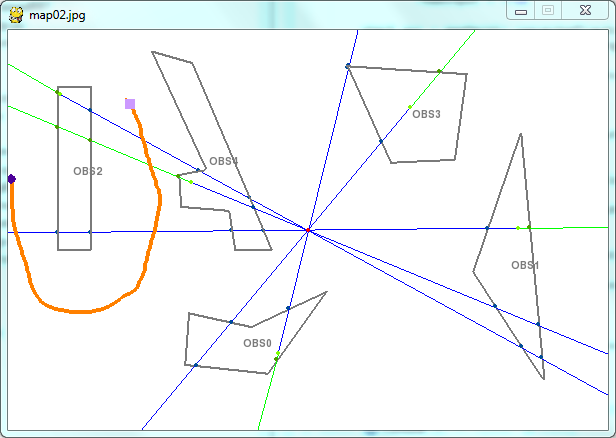
\includegraphics[width=\textwidth]{fig/referenceHomotopy.png}
		\caption{Reference path}
		\label{fig:reference_path:reference}
	\end{subfigure}  
	%\\
	\begin{subfigure}[t]{0.47\linewidth}
		\centering
		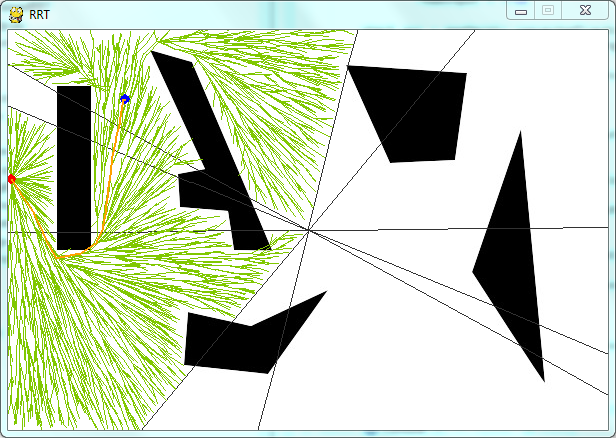
\includegraphics[width=\textwidth]{fig/homotopicConstrainedRRT.png}
		\caption{RRT$^{*}$ with homotopic constraint}
		\label{fig:reference_path:rrt}
	\end{subfigure}   
	\caption{Homotopic constraint from a reference path.}
	\label{fig:reference_path}
\end{figure}

Figure \ref{fig:reference_path} gives an example.
A user firstly initializes a reference path, which indicates the intended homotopy class as in Figure \ref{fig:reference_path:reference}.
The string of the reference path is then extracted as the constraint.
The exploration of HA-RRT$^{*}$ is then under this constraint.
Thus, in Figure \ref{fig:reference_path:rrt}, the tree only explores the regions that does not violate the grammar to generate the constraint string.

\subsection{Homotopic constraints from required/forbidden regions}

In planning a path for a task, if the human only can tell several regions that should be avoided or several regions that are required to visit, HA-RRT$^{*}$ explores the paths that satisfies the defined constraints as well.
The {\sc InitRefFrames} procedure decomposes the map and generates the topological graph, for which Figure \ref{fig:obs_map:map} gives an example.
We define the \emph{positive region} as the region that is required to visit and the \emph{negative region} as the region that is forbidden to visit.
Then there is an interactive process for the human to label the positive regions and the negative regions.
Unlabeled regions are neutral, which means no constraint here.

Because the decomposed regions are randomly and automatically generated, a decomposed region might contain both positive regions and negative regions.
In this case, the decomposed region will be split into several smaller regions so that each region might contain either positive region or negative region.
After that, more reference frames will be created correspondingly and a new topological graph will be obtained.

As each region is a node in the topological graph, the nodes of the negative regions can be trimmed firstly.
A breath first search on the topological graph can return a set of strings that satisfy the labeled constraints, which also indicates a set of homotopy classes.
The grammar is then defined by this set of strings.
The {\sc HomotopyCheck} in the exploration of HA-RRT$^{*}$ will be defined by this grammar.
The path returned by the HA-RRT$^{*}$ is the optimal solution under the labeled constraint.

\subsection{Homotopy classes with preference}

Sometimes there exists no hard constraint on the topology of the paths.
But there does exist the difference on different topology.
For example, visiting some region benefits some subtask, or going around some object enhances the task performance.

The topology can also be soft constraint.
When the user has a preference on some of the homotopy classes or all the homotopy classes,
the preference value of each homotopy class could be assigned.
In this case, the topology can be viewed as a new objective.
Each homotopy class is a value of the variable that represents the topology type.
The variable of the topology type is discrete.
The problem is converted into a two-objective optimization problem.
Because the optimal solution in a homotopy class dominates all other solutions in the homotopy class.
By combining the optimal solutions in all the homotopy classes, we can have the Pareto front of all the solution.

\begin{figure}
	\centering
	\begin{subfigure}[t]{0.47\linewidth}
		\centering
		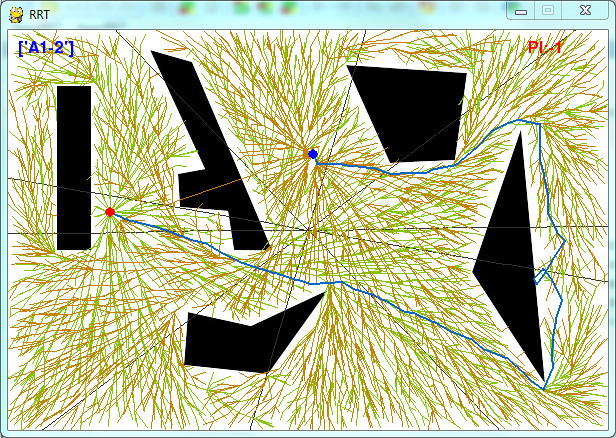
\includegraphics[width=\textwidth]{fig/homotopyClassRRT.png}
		\caption{Share same exploration space.}
		\label{fig:homotopy_no_pref:all}
	\end{subfigure}  
	%\\
	\begin{subfigure}[t]{0.47\linewidth}
		\centering
		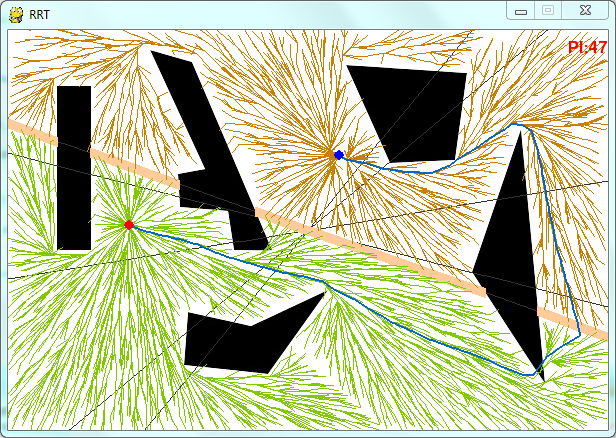
\includegraphics[width=\textwidth]{fig/homotopyClassRRTHalf.png}
		\caption{Split the exploration space.}
		\label{fig:homotopy_no_pref:half}
	\end{subfigure}   
	\caption{Bidirectional RRT$^{*}$.}
	\label{fig:homotopy_no_pref}
\end{figure}

\subsection{Homotopy classes without preference}

Sometimes inherently the user has a mind of the topology preference but feels difficult to describe.
Then, showing the optimal solution of all the homotopy classes helps the user figuring out an ``optimal'' solution that matches his inherent preference.

\begin{figure}
	\centering
	\begin{subfigure}[t]{0.47\linewidth}
		\centering
		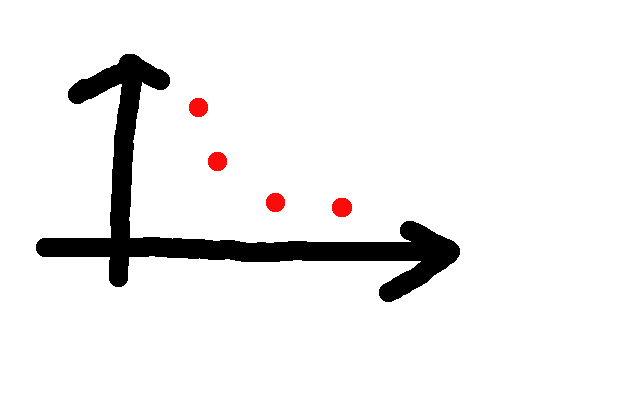
\includegraphics[width=\textwidth]{fig/pareto.png}
		\caption{Pareto front with topology preference.}
		\label{fig:homotopy_human_interaction:pareto}
	\end{subfigure}  
	%\\
	\begin{subfigure}[t]{0.47\linewidth}
		\centering
		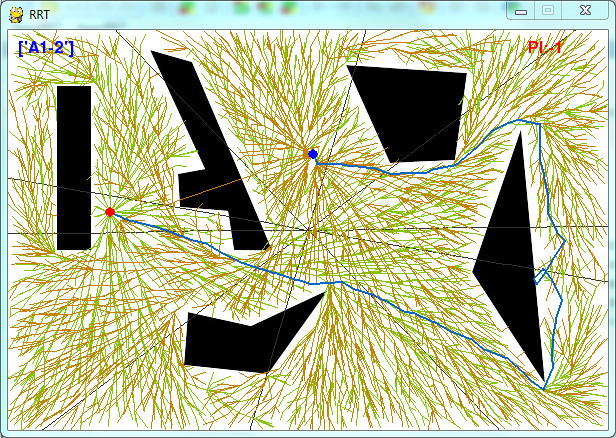
\includegraphics[width=\textwidth]{fig/navBestInHomotopy.png}
		\caption{Navigate the best solution of each homotopy class.}
		\label{fig:homotopy_human_interaction:all}
	\end{subfigure}   
	\caption{Interactive optimization.}
	\label{fig:homotopy_human_interaction}
\end{figure}


\begin{thm}
\label{thm:homotopy_no_pref:optimal}
Given Assumptions 1 - 3 in \cite{Karaman-RSS-10},

\end{thm}

\section{Analysis}
\label{sec:analysis}

The HA-RRT$^{*}$ is consist of the homotopy-aware exploration and the constrained optimization.
We look at the 
and give the constrained optimal guarantee in this section.

\subsection{homotopic grammar}

Each path or subpath can be converted into a string, which represents a sequence of characters by crossed reference frames.
The grammar of the strings could be introduced to manage the exploration process and sort the paths into different homotopy classes.

\begin{figure}
	\centering
	\begin{subfigure}[t]{0.4\linewidth}
		\centering
		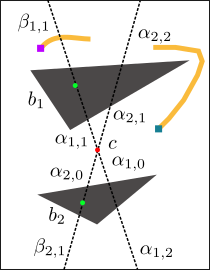
\includegraphics[width=\textwidth]{fig/feasibility}
		\caption{Feasibility}
		\label{fig:grammar:feasibility}
	\end{subfigure}  
	\begin{subfigure}[t]{0.4\linewidth}
		\centering
		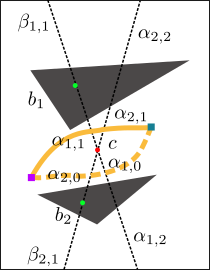
\includegraphics[width=\textwidth]{fig/equivalence}
		\caption{Equivalence}
		\label{fig:grammar:equivalence}
	\end{subfigure}
	\\
	\begin{subfigure}[t]{0.4\linewidth}
		\centering
		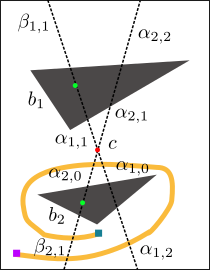
\includegraphics[width=\textwidth]{fig/recurring}
		\caption{Recurring}
		\label{fig:grammar:recurring}
	\end{subfigure}  
	\begin{subfigure}[t]{0.4\linewidth}
		\centering
		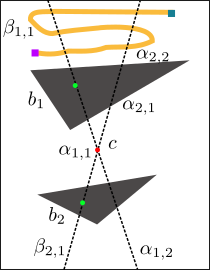
\includegraphics[width=\textwidth]{fig/repeated_pattern}
		\caption{Equivalence}
		\label{fig:grammar:repeated_pattern}
	\end{subfigure} 
	\caption{Homotopic grammar.}
	\label{fig:grammar}
\end{figure}

\begin{itemize}
\item \textbf{Feasibility}
As the reference frames are connected by the regions, a feasible string follows some grammar defined by the connectivity.

\item \textbf{Equivalence}
Some characters of the reference frames are equivalent in constructing the strings.
All the reference frames contains the center point $ c $ show this property.
The segment crossing those reference frames in any sequence belongs to same homotopy class.


\item \textbf{Recurring character}
Recurring character in a string indicates that the path goes around some obstacles and back to a visited region.


\item \textbf{Repeated pattern}
Repeated pattern shows that the path is back and forth among some regions.

\end{itemize}

\subsection{Optimality with constraint}

We can have the asymptotic optimality with the constraint of via-points.
It is stated in Lemma \ref{lem:optimal_via_point}.

\begin{lem}
\label{lem:optimal_via_point}
Given Assumptions 1 - 3 in \cite{Karaman-RSS-10},
the path concatenated from a path from $ G_{s} $ for $ v $ and a path from $ G_{g} $ for $ v $ converges to the optimal path through $ v $ almost surely. 
\begin{proof}
\end{proof}
\end{lem}

\begin{thm}
\label{thm:constrained_optimality}
Given Assumptions 1 - 3 in \cite{Karaman-RSS-10},
\end{thm}

\subsection{Discussion}

Dilemma between efficiency and scenario support

\subsubsection{Scenario support}

\subsubsection{Efficiency}

\section{Conclusion}
\label{sec:conclusion}

\bibliographystyle{IEEEtranS}
\bibliography{reference}

\end{document}